\message{ !name(main.tex)}%%%%%%%%%%%%%%%%%%%%%%%%%%%%%%%%%%%%%%%%%
% Masters/Doctoral Thesis
 
% Version 1.43 (17/5/14)
%
% This template has been downloaded from:
% http://www.LaTeXTemplates.com
%
% Original authors:
% Steven Gunn 
% http://users.ecs.soton.ac.uk/srg/softwaretools/document/templates/
% and
% Sunil Patel
% http://www.sunilpatel.co.uk/thesis-template/
%
% License:
% CC BY-NC-SA 3.0 (http://creativecommons.org/licenses/by-nc-sa/3.0/)
%
% Note:
% Make sure to edit document variables in the Thesis.cls file
%
%%%%%%%%%%%%%%%%%%%%%%%%%%%%%%%%%%%%%%%%%



%%----------------------------------------------------------------------------------------
%	PACKAGES AND OTHER DOCUMENT CONFIGURATIONS
%----------------------------------------------------------------------------------------

\documentclass[11pt, oneside]{Thesis} % The default font size and one-sided printing (no margin offsets)

\graphicspath{{Pictures/}} % Specifies the directory where pictures are stored
%\usepackage{xparse}
%\usepackage{physics}
%\usepackage{braket,mleftright}
%\mleftright
\usepackage[square, numbers, comma, sort&compress]{natbib} % Use the natbib reference package - read up on this to edit the reference style; if you want text (e.g. Smith et al., 2012) for the in-text references (instead of numbers), remove 'numbers' 
%\usepackage{txfonts}
\hypersetup{urlcolor=blue, colorlinks=true} % Colors hyperlinks in blue - change to black if annoying
\title{\ttitle} % Defines the thesis title - don't touch this
\usepackage{relsize}
\usepackage{amsmath}
\usepackage{adjustbox}
\usepackage{leftidx}
\usepackage{auctex}

    \newenvironment{dedication}
        {\vspace{6ex}\begin{quotation}\begin{center}\begin{em}}
        {\par\end{em}\end{center}\end{quotation}}

\newcommand*{\defeq}{\mathrel{\vcenter{\baselineskip0.5ex \lineskiplimit0pt
                     \hbox{\scriptsize.}\hbox{\scriptsize.}}}%
                     =}


\newcommand{\veq}{\mathrel{\rotatebox{90}{$=$}}}
\newcommand{\vneq}{\mathrel{\rotatebox{90}{$\neq$}}}

\renewcommand{\bibname}{References}

\begin{document}

\message{ !name(main.tex) !offset(-3) }


\frontmatter % Use roman page numbering style (i, ii, iii, iv...) for the pre-content pages

\setstretch{1.25} % Line spacing of 1.3

% Define the page headers using the FancyHdr package and set up for one-sided printing
\fancyhead{} % Clears all page headers and footers
\rhead{\thepage} % Sets the right side header to show the page number
\lhead{} % Clears the left side page header

\pagestyle{fancy} % Finally, use the "fancy" page style to implement the FancyHdr headers

\newcommand{\HRule}{\rule{\linewidth}{0.5mm}} % New command to make the lines in the title page

% PDF meta-data
\hypersetup{pdftitle={\ttitle}}
\hypersetup{pdfsubject=\subjectname}
\hypersetup{pdfauthor=\authornames}
\hypersetup{pdfkeywords=\keywordnames}

%----------------------------------------------------------------------------------------
%	TITLE PAGE
%----------------------------------------------------------------------------------------

\begin{titlepage}
\begin{center}

%\textsc{\LARGE \univname}\\[1.5cm] % University name
%\textsc{\Large MPhys Thesis}\\[0.5cm] % Thesis type

\HRule \\[0.4cm] % Horizontal line
{\Large \bfseries \ttitle}\\[0.4cm] % Thesis title
\HRule \\[1.5cm] % Horizontal line
 
\begin{minipage}{0.4\textwidth}

%\emph{Author:}\\
%\href{mailto:anon@cam.ac.uk}{\authornames} % Author name - remove the \href bracket to remove the link
\end{minipage}
\begin{minipage}{0.4\textwidth}
\begin{flushright} \large
%\emph{Supervisors:} \\
%{\supname} % Supervisor name - remove the \href bracket to remove the link  
\end{flushright}
\end{minipage}\\[1cm]

\begin{center}
Nick Woods
\end{center} \large

\vspace{2cm}

%\begin{figure}[h]
%   \centering
%   \includegraphics[scale=0.08]{CambCrest}
%\end{figure}
%\begin{figure}[h]
%   \centering
%   \includegraphics[scale=0.5]{logo}
%\end{figure}

\vspace{3cm}

%\large \textit{An essay submitted in fulfilment of the requirements\\ for the degree of \degreename}\\[0.3cm] % University requirement text
%\textit{in the}\\[0.2cm]
%\deptname \\ % Research group name and department name
 
\vspace{8cm}

{\large \today} % Date


\vfill
\end{center}

\end{titlepage}





%----------------------------------------------------------------------------------------
%	QUOTATION PAGE
%----------------------------------------------------------------------------------------

%\pagestyle{empty} % No headers or footers for the following pages

%\null\vfill % Add some space to move the quote down the page a bit

%\textit{``You miss 100$\%$ of the shots you don't %take"}

%\begin{flushright}
%Wayne Gretzky\end{flushright}

%\vfill\vfill\vfill\vfill\vfill\vfill\null % Add some space at the bottom to position the quote ust right

%\clearpage % Start a new page


%
%----------------------------------------------------------------------------------------
%	LIST OF CONTENTS/FIGURES/TABLES PAGES
%----------------------------------------------------------------------------------------

\pagestyle{fancy} % The page style headers have been "empty" all this time, now use the "fancy" headers as defined before to bring them back

\lhead{\emph{Contents}} % Set the left side page header to "Contents"
\tableofcontents % Write out the Table of Contents

%----------------------------------------------------------------------------------------
%	THESIS CONTENT - CHAPTERS
%----------------------------------------------------------------------------------------



\mainmatter % Begin numeric (1,2,3...) page numbering

\pagestyle{fancy} % Return the page headers back to the "fancy" style

% Include the chapters of the thesis as separate files from the Chapters folder
% Uncomment the lines as you write the chapters

\makeatletter
\def\@makechapterhead#1{%
  \vspace*{50\p@}%
  {\parindent \z@ \raggedright \normalfont
    %\ifnum \c@secnumdepth >\m@ne
    %    \huge\bfseries \@chapapp\space \thechapter
    %    \par\nobreak
    %    \vskip 20\p@
    %\fi
    \interlinepenalty\@M
    \Huge \bfseries #1\par\nobreak
    \vskip 40\p@
  }}
  \makeatother

\renewcommand{\chaptername}{}

% Chapter 1

\chapter{Introduction} % Main chapter title

\label{Chapter2} % For referencing the chapter elsewhere, use \ref{Chapter1} 

\lhead{2. \emph{Introduction}} % This is for the header on each page - perhaps a shortened title


% Chapter 1

\chapter{Theory} % Main chapter title

\label{Chapter1} % For referencing the chapter elsewhere, use \ref{Chapter1} 

\lhead{1. \emph{Theory}} % This is for the header on each page - perhaps a shortened title

%----------------------------------------------------------------------------------------
\section{The Problem}

\label{sec21}

Solving a set of non-linear equations is the final step in the solution of many practical problems in Physics. This can be formulated as finding the `fixed point' of a multidimensional function
\begin{align}
\textbf{g}(\textbf{x}^*) = \textbf{x}^*,
\end{align}
or recast as a root finding problem
\begin{align}
\label{root}
\textbf{f}(\textbf{x}^*) = \textbf{g}(\textbf{x}^*) - \textbf{x}^* = \textbf{0} 
\end{align}
i.e. find $\textbf{x}^* \in \mathbb{R}^n$ such that the function $\textbf{f} : \mathbb{R}^n \rightarrow \mathbb{R}^n$, defined above, is zero. Fixed point iteration theory states that for a sufficiently well behaved (continuous, etc.) function and input argument, the iterative process $\textbf{g}(\textbf{x}_n) = \textbf{x}_{n+1}$ will converge with some order of convergence. The convergence (both speed and success) of a less well behaved operation than the $\textbf{g}$ above can be improved beyond fixed point iterations if $\textbf{x}_{n+1}$ is chosen `well'. That is, if one chooses $\textbf{x}_{n+1} = \textbf{h}(\textbf{g}(\textbf{x}^{\text{in}}_n) = \textbf{x}^{\text{out}}_{n}, \textbf{x}_n^{\text{in}})$ with $\textbf{h}$ a function defined to assist convergence toward Eq$.$ (\ref{root}). All methods below seek to find the form of $\textbf{h}$ such that Eq$.$ (\ref{root}) can be achieved, and be achieved as fast as possible in the specific case of Kohn-Sham DFT.

The above can now be rearranged in terms of Kohn-Sham (KS) DFT. The KS Hamiltonian, $H^{\text{ks}}$, solves an eigenproblem,
\begin{align}
\label{KSH}
H^{\text{ks}} \psi_i = \epsilon_i \psi_i. 
\end{align} 
However, one finds that the solutions, $\psi_i$, depend on the input, $H^{\text{ks}}$, through the electron density -- $H^{\text{ks}} = H^{\text{ks}}[\rho]$ where,
\begin{align}
\label{rout}
\rho(\textbf{r}) = \sum_{i \in \text{occupied}} |\psi_i(\textbf{r})|^2.
\end{align} 
Hence, the above process (Eq$.$ (\ref{KSH}) and Eq$.$ (\ref{rout})) can be compacted into a \textit{self-consistent field operator} $F$, satisfying
\begin{align}
F[\rho^{\text{in}}] = \rho^{\text{out}}. 
\end{align} 
The $\rho^*$ that satisfies both Eq$.$ (\ref{KSH}) and Eq$.$ (\ref{rout}), i.e. $\rho^{\text{in}} = \rho^{\text{out}}$, is the electron density that solves KS DFT for a given external potential, system size, etc. One now seeks the function $\textbf{h}(\rho^{\text{in}}, \rho^{\text{out}})$ such that $\rho^{\text{in}} = \rho^{\text{out}}$ is satisfied (within some tolerance) as quickly and robustly as possible -- `\textit{density mixing}'.  The corresponding function to $\textbf{f}$ in Eq$.$ (\ref{root}) is now defined as the \textit{residual} -- $R[\rho(\textbf{r})] =  \rho^{\text{in}} - \rho^{\text{out}}$, where $\textbf{h}$ drives $R$ toward zero, thus finding the ground state electron density $\rho^*$ ($R[\rho^*] = 0$). A few `problem dependent' properties can now be noted: firstly, the evaluation of the operation $F$ is extremely costly, as it involves (iterative) diagonalisation of an $N_{\text{pw}} \times N_{\text{pw}}$ matrix. This means one would favour a density mixing scheme which converges in a low iteration count, at the cost of many computations per iteration (to an extent). Furthermore, the analytic form of the derivative $\partial_{\rho} F$ is not readily available, meaning some finite-differenced numerical approximation will be often need to be computed (atleast for the first step in an iterative process). This derivative -- the Jacobian -- is conventionally stored in a matrix which is prohibitively large (size dependent on the discretisation of the space), both in terms of computation cost and in storage requirements (when applying some mixing scheme). One therefore seeks a density mixing scheme which can be executed with limited memory requirements (i.e. not storing such large matrices), and converges in a low number of SCF cycles. With this in mind, the difficulties in applying some of the `naive' approaches to the SCF process can be outlined. 








\section{Characterisation of the Solutions}


The simplest update to the density would be to treat the above system as a fixed point iteration, feeding the output density back in as the input density by computing $\rho_{n+1}=F[\rho_{n}]$ -- this turns out to be unsuitable for a variety of reasons. To elaborate, first note that the iterates will take the form $\rho^{\text{in}}_{n+1} = \rho^{\text{out}}_{n} = F[\rho^{\text{in}}_{n}]$. In practice, the initial guess of the density is not far from the converged density by simply modelling atoms at $\textbf{R}_{\mu}$ as pseudoatomic orbitals of charge at $\textbf{R}_{\mu}$. This can be seen in Fig$.$ \ref{convergence}, where a bulk FCC Al structure took 5 SCF iterations to converge within tolerance. By-eye inspection reveals that the initial guess does not change much from the converged density, and in fact after only one iteration the densities become visually indistinguishable as plotted. If it is the case that the $\rho^{\text{initial guess}} \sim \rho^*$ the operation $F$ can be linearised about $\rho^*$,
\begin{gather}
\rho^* + \delta \rho^{\text{out}}_n = F[\rho^* + \delta \rho^{\text{in}}_{n}] \approx F[\rho^*] + \frac{\delta F}{\delta \rho}\bigg\rvert_{\rho^*} \delta \rho^{\text{in}}_{n} = \rho^* + \frac{\delta F}{\delta \rho}\bigg\rvert_{\rho^*}  \delta \rho^{\text{in}}_{n}, \\ \label{linearresponse}
\implies \delta \rho^{\text{out}}_n = \frac{\delta F}{\delta \rho}\bigg\rvert_{\rho^*}  \delta \rho^{\text{in}}_{n}, \\
\implies \delta \rho^{\text{in}}_{n+1} = \frac{\delta F}{\delta \rho}\bigg\rvert_{\rho^*}  \delta \rho^{\text{in}}_{n}.
\end{gather}
\begin{figure}
{\hspace{-1em}}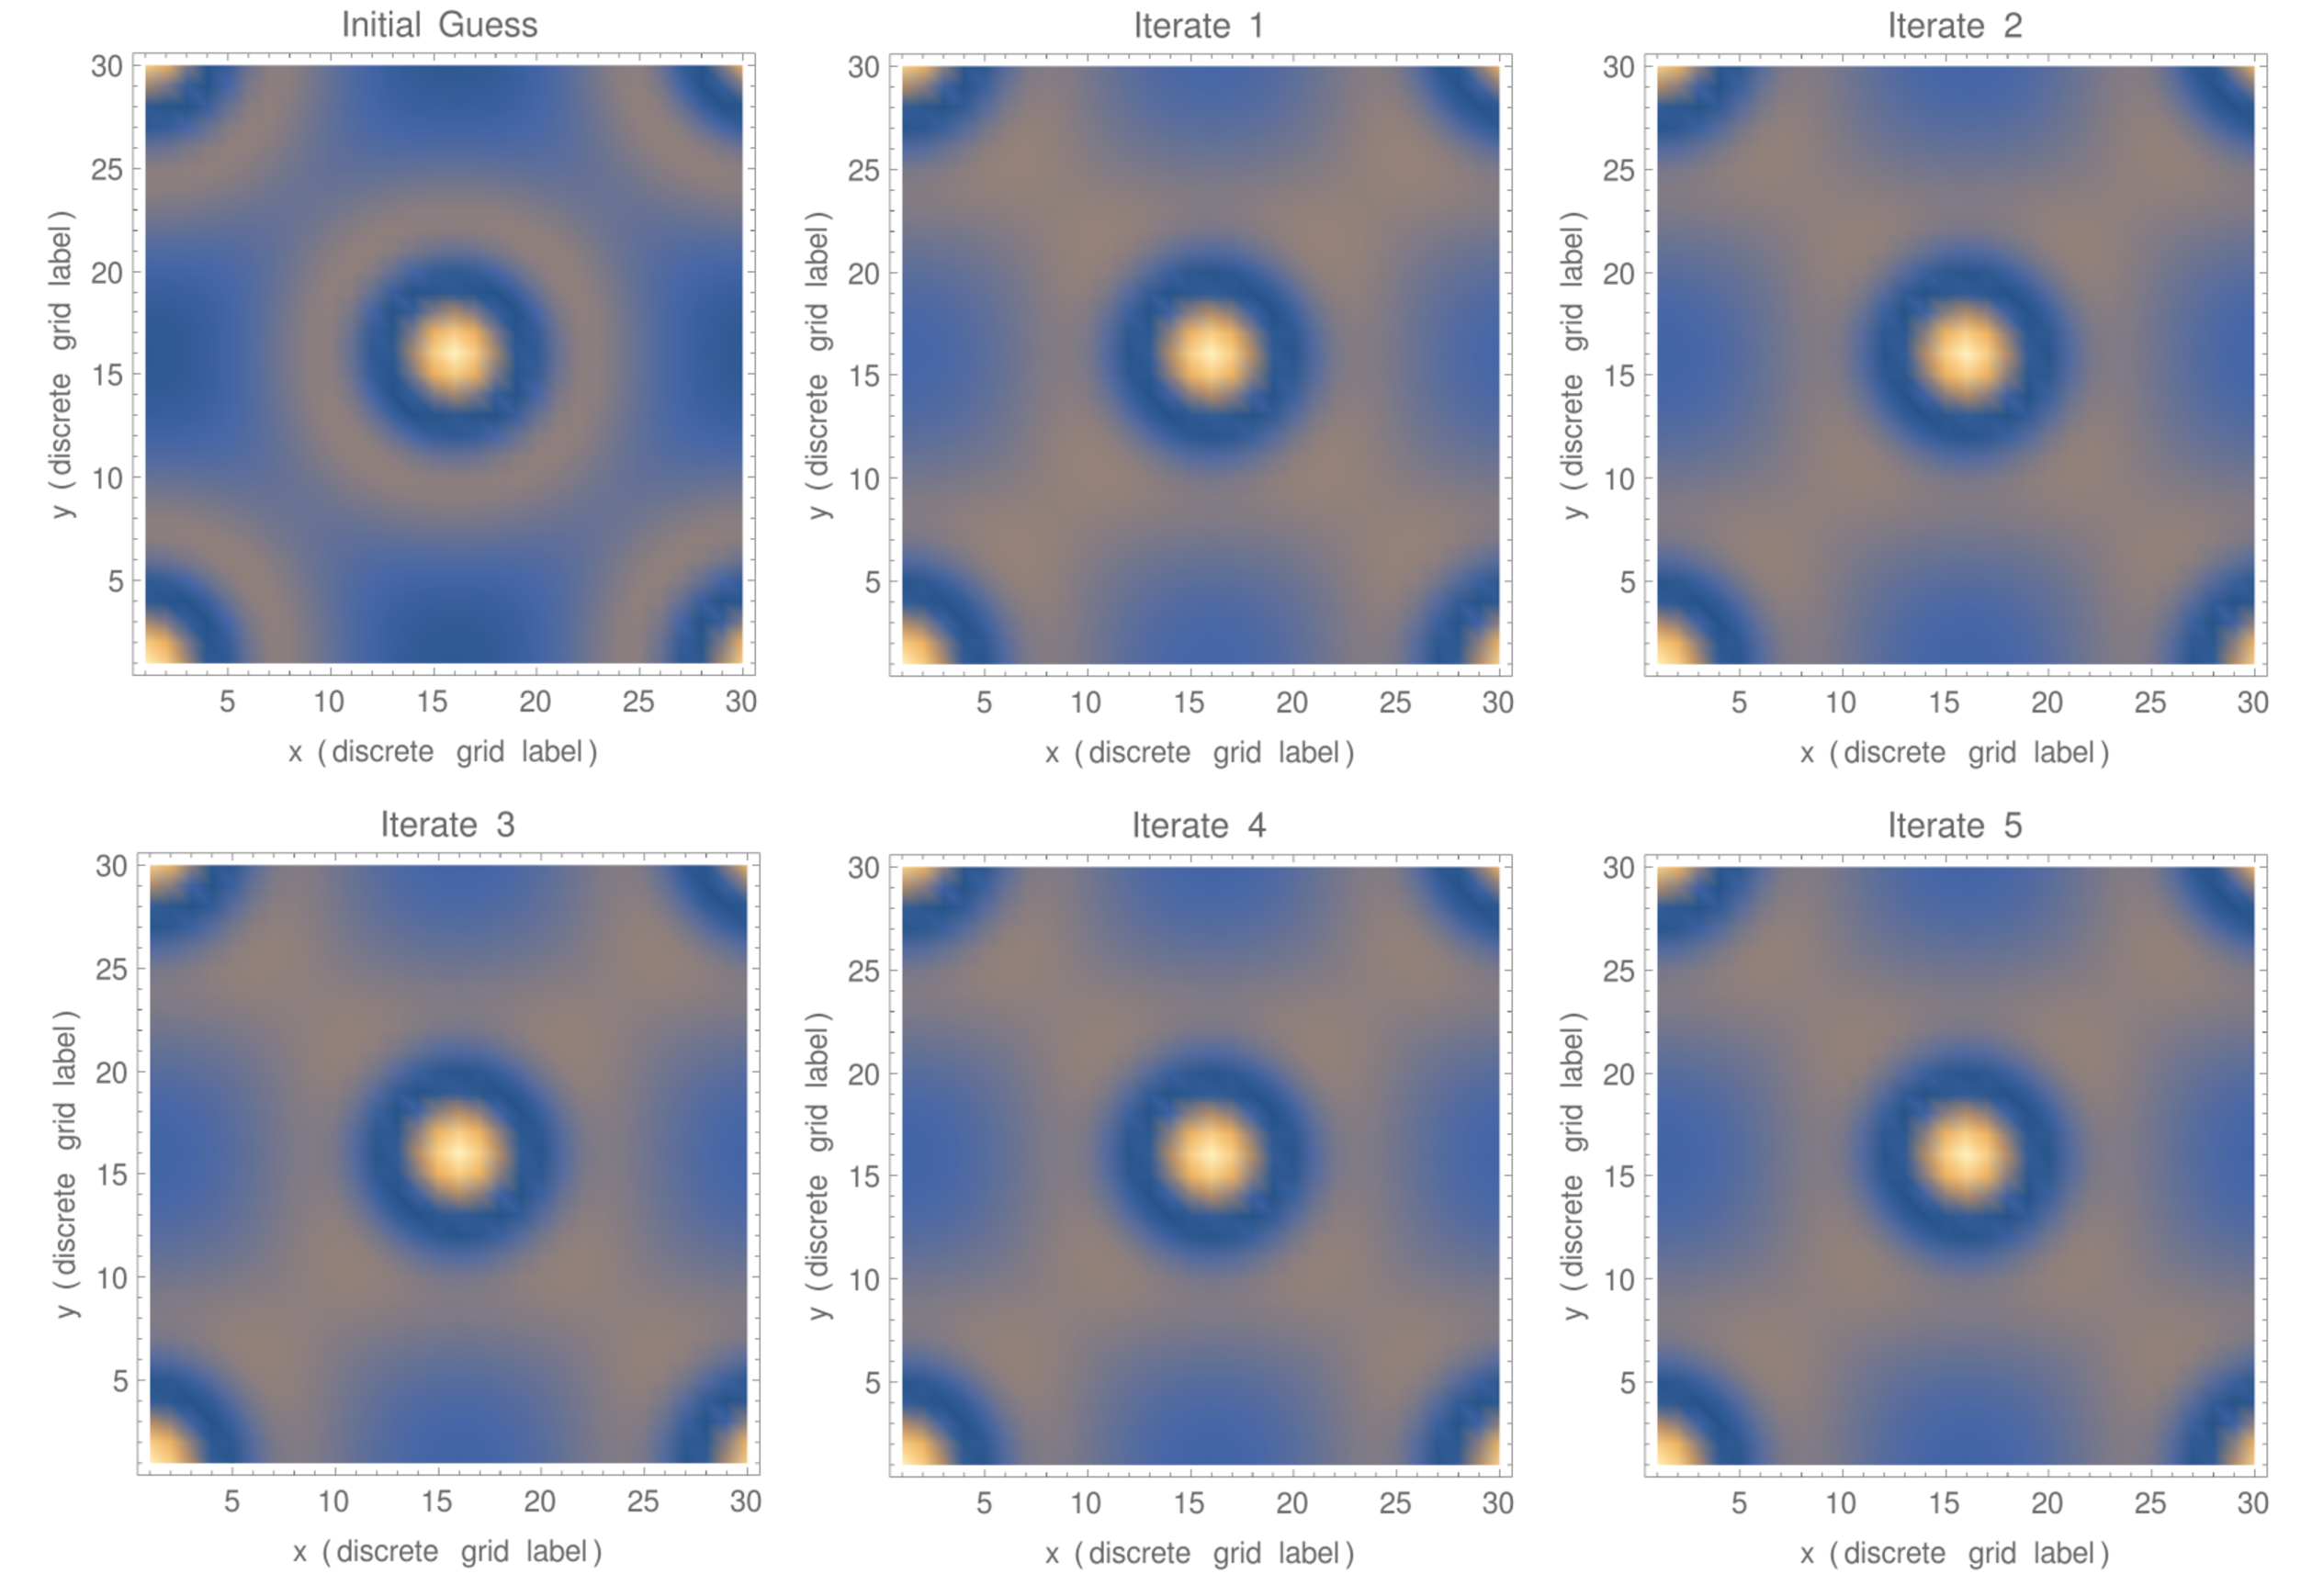
\includegraphics[width=6in]{Al_convergence.pdf}
\caption{SCF convergence of FCC aluminium in CASTEP using Pulay mixing.}
\label{convergence}
\end{figure}
Any use of Eq$.$ (\ref{linearresponse}) denotes a density mixing scheme in the \textit{linear response regime} -- i.e. it is assumed that small perturbations to the input charge density of KS DFT depend linearly on the output charge density. In general this clearly doesn't hold, but as mentioned, for charge densities sufficiently close to convergence, the relation is a good approximation. $F : \mathbb{R}^3 \rightarrow \mathbb{R}^3$ and $\rho \in \mathbb{R}^3$, so the derivative term at a point \textbf{r},\textbf{r}' in real space (ignoring any discritisation of the domain) will be a matrix $\frac{\delta F}{\delta \rho} \sim M \in \mathbb{R}^{3 \times 3}$. It will later be shown that $M$ is closely related to the DFT dielectric response of the input system. From a mathematical perspective, one can ask what the conditions on $M$ are to guarantee convergence. Convergence is defined as $\delta \rho^{\text{in}}_{n+1} \rightarrow 0$ as $n \rightarrow \infty$, or
\begin{gather}
M   \delta \rho^{\text{in}}_{n} = (M)^n \delta \rho^{\text{in}}_{1} \rightarrow 0.
\end{gather}
It will be assumed here (although it can be shown \citep{linear}) that $M$ is of full rank, and can be diagonalised using $\{  \textbf{e}_i \}$ as an orthonormal basis -- $M^d_{ij} =  \delta_{ij} \lambda_i | \textbf{e}_i \rangle \langle \textbf{e}_j |$ with $\{ \lambda_i \}$ the spectrum of $M$\footnote{Here, $M^d$ is a transformed matrix sharing some of the same properties of $M$, namely, $M^n \rightarrow 0$ iff $(M^d)^n \rightarrow 0$.}. Since $\langle \textbf{e}_i | \textbf{e}_j \rangle = \delta_{ij}$,
\begin{gather}
((M^d)^n)_{ii} = (\lambda_i)^n   | \textbf{e}_i \rangle \langle \textbf{e}_i |, \\
\implies M \delta \rho^{\text{in}}_n \rightarrow 0 \text{ iff } | \lambda_i | < 1 \text{ } \forall \text{ } i.
\end{gather} 
The question now becomes, for typical DFT input systems, is the condition $ | \lambda_i | < 1 $ always satisfied? The answer is no, and for some illustrative models studied in Ref$.$ \citep{linear} $| \lambda_i | \sim 100$, causing a strong divergence from $\rho^*$. Clearly a simple fixed point iteration-esque update to $\rho_{n+1}$ is unsuitable in general DFT calculations. It seems natural to now ask how one could incorporate a parameter to suppress $| \lambda_i |$ such that it satisfies the convergence criteria for any system of interest. This leads to the most simple density mixing scheme able to converge a (not-so-wide) variety of input systems -- \textit{linear mixing}. Instead of using $\rho^{\text{in}}_{n+1} = \rho^{\text{out}}_{n}$, one incorporates a damping parameter $\alpha$ as such,
\begin{gather}
\rho^{\text{in}}_{n+1} =  \rho^{\text{in}}_{n} + \alpha ( \rho^{\text{out}}_{n} -  \rho^{\text{in}}_{n} ) =  \rho^{\text{in}}_{n} + \alpha R[\rho^{\text{in}}_{n}].
\end{gather}
It can be seen that, defining convergence of $\delta \rho$ similarly to above, the convergence criteria now becomes $|1+\alpha (\lambda_i - 1)|<1$. As $\alpha$ can be arbitrarily tuned such that this is true, the problem has been (superficially) solved. Supposing $M$ is positive definite (i.e. not worrying about the case of $\lambda_{\text{min}}<0$), $\alpha$ must be chosen such that $|1+\alpha(\lambda_{\text{max}} - 1)| < 1$, meaning $\rho$ is guaranteed to converge for all $\lambda_i$. However, the speed of convergence is related to how close $|1+\alpha(\lambda_{\text{max}} - 1)|$ is to unity -- if it is only slightly less, $|1+\alpha(\lambda_{\text{max}} - 1)|^n$ will take large $n$ to reach zero within tolerance. Moreover, if $\alpha$ is too low, the change in the $\rho_{n+1}$ becomes minuscule per iteration for eigenvalues at or close to $\lambda_{\text{min}}$, leading to slow convergence. Therefore, an optimal value of $\alpha$ must be deduced, but how efficacious this choice is clearly depends on the ratio $\frac{\lambda_{\text{max}}}{\lambda_{\text{min}}}$ -- an important quantity in numerical analysis, the \textit{condition number} of $M$. In general $M$ is not well conditioned, e.g. for metallic materials the condition number of $M$ turns out to be divergent proportional to the size of the unit cell [source?], and hence certain systems can take large amounts of time to converge (to the point where a user would say the calculation doesn't converge in a practical sense).

The above discussion on the convergence of fixed point iterations and linear mixing was mathematical in nature, but the lack of convergence of both methods can also be interpreted physically in a process dubbed `charge sloshing'. One starts by interpreting $M = \frac{\delta F}{\delta \rho}$ in Eq$.$ (\ref{linearresponse}). The functional derivative of the operator $F$ has been investigated by multiple sources \citep{linear,Fderiv}, and it can be shown that $M$ relates to the dielectric constant matrix $\epsilon$ in the following way,
\begin{gather}
M = \textbf{I} - \epsilon^{\text{DFT}}.
\end{gather}
The dielectric describes how the electrons in a given system will respond to an (applied) perturbation in the electron density -- $\frac{\delta \rho^{\text{out}}}{\delta \rho^{\text{in}}}$. Applying a perturbation to the electron density amounts to mimicking the application an external electric field, and measuring the response of the electrons (which is the classical electromagnetism definition of a dielectric). It will be shown below that knowing the dielectric of the input system can greatly improve convergence to the ground state, firstly however a subtle but important distinction can be made. When one says `the dielectric of the input system', what is meant by this is the dielectric of the input system \textit{as it would be in} KS DFT. The idea of density mixing is to converge KS DFT to its ground state as quickly as possible, and the dielectric that is most efficacious in achieving this is not the dielectric of the real material, but the dielectric as it would be in KS DFT\footnote{Obviously these are ideally the same, but it is unfortunately not always the case.}. This fact becomes not so subtle when the dielectric (or some other mathematical object designed to assist convergence) requires the \textit{band gap} as a parameter. One might initially (correctly) identify that DFT systematically underestimates the band gap, and then (incorrectly) deduce that convergence processes relying on the band gap are unsuitable (or at the very least non-optimal). However, it is precisely the DFT band gap that is required for optimal performance, as density mixing is a numerical technique designed to extract the correct output answer from the theory.

Analysis in \citep{Fderiv2} confirms that \textit{at the fixed point} $\rho^*$, $\epsilon$ (and therefore $M$) is positive definite as presumed (which removes some divergence possibilities, allowing $\alpha$ to remain positive). Breaking down $\epsilon$ component by component reveals that perturbations in the charge density and \textit{Hartree} potential\footnote{Ignoring the exchange-correlation component for now, as it does not affect the ensuing analysis.} affect one-another as so,
\begin{gather}
\delta V_h(\textbf{r}) = \int \frac{\delta \rho(\textbf{r}')}{|\textbf{r} - \textbf{r}'|} \text{ } d\textbf{r}', \label{slosh1} \\
\delta \rho(\textbf{r}) = \int \chi^{\text{DFT}} (\textbf{r},\textbf{r}') \delta V_h(\textbf{r}') \text{ } d\textbf{r}'. \label{slosh2}
\end{gather}
In this context, $\chi^{\text{DFT}}$ is the independent (DFT) electron \textit{susceptability} -- a real, symmetric matrix characterising how `susceptible' the electrons in an input system are to changes in the potential, $\chi^{\text{DFT}} \sim \frac{\delta \rho}{\delta V_h}$. One can see that $M$ will pick up amplified contributions from changes in the charge density at long range from Eq$.$ (\ref{slosh1}). In Fourier space, Eq$.$ (\ref{slosh1}) takes the form,
\begin{gather}
\delta \tilde{V}_h(\textbf{G}) \sim \frac{\delta \tilde{\rho}(\textbf{G})}{|\textbf{G}|^2}.
\end{gather}
Hence, finite changes in the density at short wavelength Fourier modes ($\delta \rho$ at long range in real space) will be amplified by the factor of $|G|^{-2}$. This then has a back-reaction on the iteratively updated output density, Eq$.$ (\ref{slosh2}). Depending on the susceptibility, a large change will be incurred in $\delta \rho^{\text{out}}_{n+1}$, and the system will fail to converge. The dependence on $\chi$ (and therefore $\epsilon$) is the link between the mathematical analysis above, and the discussion here. If the maximum eigenvalue of $U \chi$ -- U being the kernel of the Hartree potential -- is too large (or the spectrum is not dense in the linear mixing case), the electrons are `too' susceptible to changes in the potential causing divergence (or extremely slow convergence). The physical picture being that, when the material is `too' susceptible (relating to the eigenvalues of $\chi$) a small change in the Hartree potential (for example the one induced in the mixing schemes) causes a large change in the charge density from low $|G|$ wavevectors. This in turn back-reacts onto $V_h$ trying to accommodate for the change in $\rho$, which sets up a `back-and-forth' of continuous overcorrection of $\rho$ and $V_h$ -- sloshing. Unfortunately, charge sloshing is present in all mixing algorithms to an extent, where the effect is more pronounced in high $\chi$ materials, like metals, and particularly when the unit cell (and charge inside the cell) is large\footnote{It seems intuitive that for more charge present over longer ranges, the sloshing will be more pronounced.}. In reference to the earlier discussion, the reason why Ref$.$ \citep{linear} finds $\lambda_i \sim 100$ is precisely because they are modelling a metallic system whose electrons respond much more freely to the `applied field' in contrast to an insulating system. 

Charge sloshing can be seen in action in Fig$.$ \ref{sloshing}. A graphene nanoribbon consisting of 12 atoms was attempted to be converged using linear mixing (and for reference, actually converged using Pulay mixing in Fig$.$ \ref{sloshing2}). This system is (semi-)metallic, and has a large unit cell in the plotted direction (across the ribbon) as it includes 10\AA \text{ } of vacuum space. It can be seen that the initial guess, as expected, is close to the converged answer (when comparing to the Pulay case). However, after just two iterations, large amounts of charge starts getting displaced per iteration. The mixing algorithm attempts to move charge to the edge of the unit cell, and then overcorrects in the next iteration by moving all charge to the centre of the unit cell. What is left by iteration five does not resemble the input system at all, and hence the instability has taken over and linear mixing has failed to converge.  
\begin{figure}
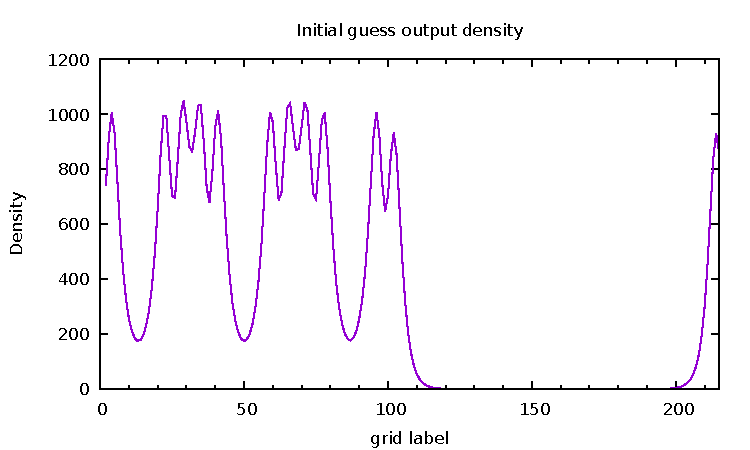
\includegraphics[width=2.8in]{Pictures/slosh1.pdf}
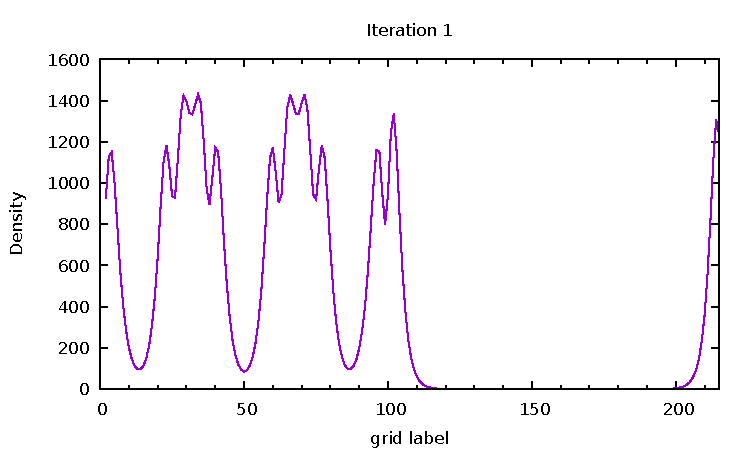
\includegraphics[width=2.8in]{Pictures/slosh2.pdf}
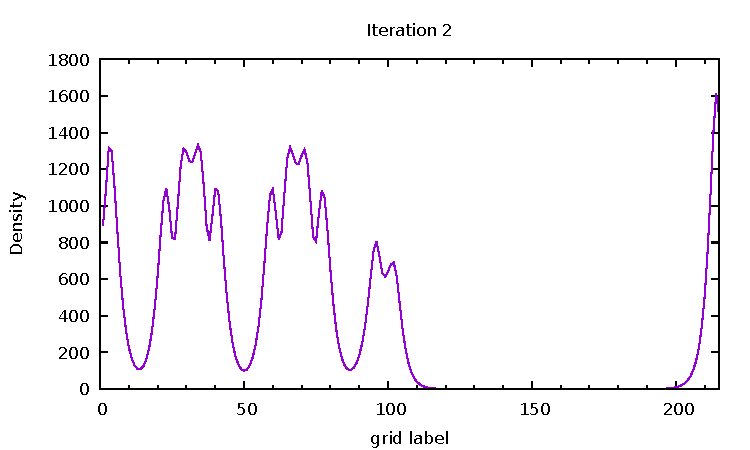
\includegraphics[width=2.8in]{Pictures/slosh3.pdf}
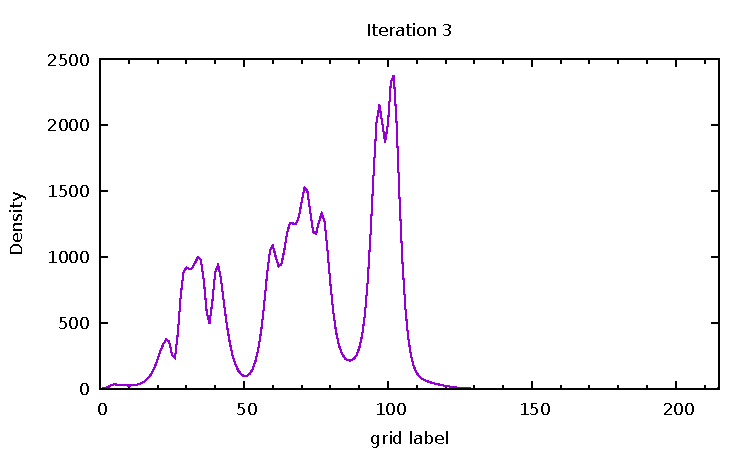
\includegraphics[width=2.8in]{Pictures/slosh4.pdf}
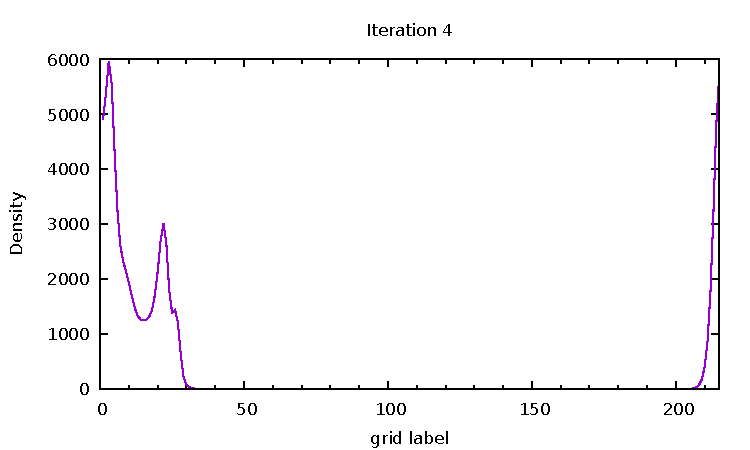
\includegraphics[width=2.8in]{Pictures/slosh5.pdf}
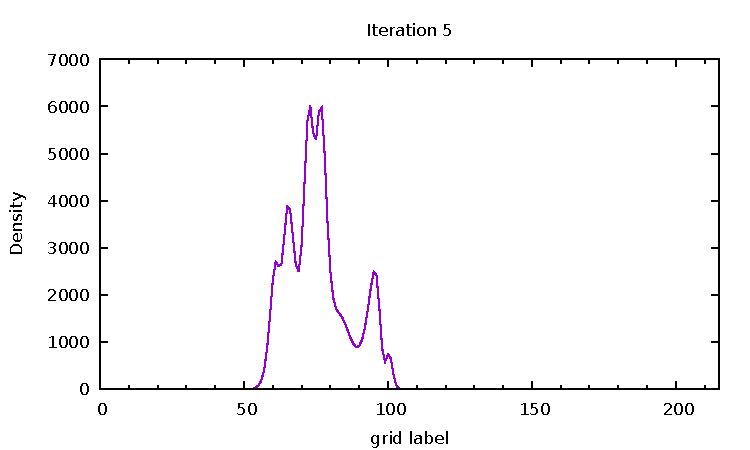
\includegraphics[width=2.9in]{Pictures/slosh6.pdf}
\caption{Electron densities at subsequent iterations of the SCF process for a 12 atom ZGNR using linear mixing.}
\label{sloshing}
\end{figure}
\begin{figure}
\centering
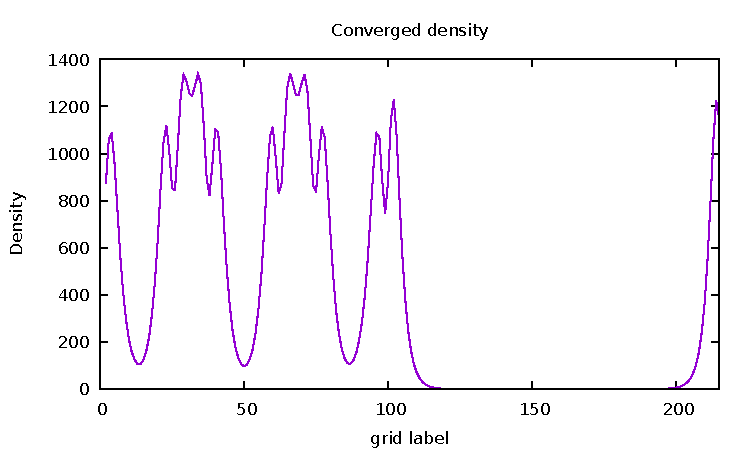
\includegraphics[width=3.5in]{Pictures/pulay_converged.pdf}
\caption{Converged electron density for a 12 atom ZGNR using Pulay mixing.}
\label{sloshing2}
\end{figure}



Another source of what one could interpret as a sloshing instability is related to how KS orbital occupations are determined for systems where the Fermi energy crosses the bands (metallic systems again, but for differing reasons to above). In a DFT calculation the software will converge the total energy,
\begin{gather}
E_{\text{tot}} = \sum_{i \in \text{occupied}} \epsilon_i - \text{double counting},
\end{gather}
where occupation refers to the electrons in the system occupying specific single particle KS orbitals $\phi_i$ with energy $\epsilon_i$ such that $E_{\text{tot}}$ is minimised. In semiconductors and insulators, determination of the occupation is simple: it is discontinuous and the lowest energy $N$ orbitals are filled with electrons, and any bands above $E_f$ (which are completely separate to bands below $E_f$) have their corresponding orbitals unoccupied. In metals however, the bands cross at $E_f$ and the act of choosing (discontinuously) one of the orbitals to be fully occupied, and the other to be not occupied, can raise the energy of the occupied band over the previously unoccupied one in the next SCF iteration. The DFT program will then choose the previously unoccupied orbital to now be the occupied orbital, and thus the process repeats and convergence of $E_{\text{tot}}$ may never be reached. This form of sloshing is less serious than the sloshing as a product of $V_h$ and $\chi$, as one can introduce a fix in the form of \textit{partial occupancy}. In implementing this, the occupancy of orbitals with energies around $E_f$ are no longer discontinuous, but smeared according to some `finite temperature' distribution $f_i$ (e.g. Fermi-Dirac), allowing $E_{\text{tot}}$ to be converged much more systematically and reliably by the code. 

This first form of sloshing is atleast partially solved by the use of a model dielectric. In practice, the model dielectric matrix $\sim M$ is applied to the electron density in Fourier space, and is specifically designed to weight changes of $\rho$ at low $|G|$ less, heavily damping the sloshing effect. In mathematical terms, the dielectric matrix acts as a \textit{preconditioner}, which takes the problem at hand (i.e. driving $\rho^{\text{guess}} \rightarrow \rho^*$) and changes the problem (by application of the preconditioner) to make it more suitably solved by the mixing algorithm.

The above analysis has highlighted two key considerations when seeking to improve the SCF cycles in KS DFT -- the choice of mixing algorithm, and the choice of preconditioner. It is common in practice to apply the preconditioner at each iteration of the mixing algorithm (specified by $\textbf{h}$). Now the base theory has been laid out, one can begin to seek so-called \textit{advanced mixing} algorithms to assist convergence, and improved preconditioners/dielectric models. 




\section{Improving the SCF Process}

\subsection{Advanced Density Mixing}

Firstly a range of mixing methods will be introduced and detailed in (almost) chronological order, with the goal of arriving at the methods currently implemented in CASTEP. The methods below can be categorised into two broad classes: \textit{direct inversion of the iterative subspace} (DIIS) -- a method using a history of iterates to perform a least squares weighting of the subsequent iterate in order to achive zero `error' -- and quasi-Newton methods. The foundation of quasi-Newton techniques is the Newton-Raphson method for approximating roots, which will first be outlined. 

\subsubsection{Newton's Method}

As discussed, the SCF solution of KS DFT is a root finding problem, requiring $R[\rho^*]=0$. Reintroducing the mathematical notation from the start of Section$.$ \ref{sec21}, Newton's method for finding $\textbf{x}^*$ such that $\textbf{f}(\textbf{x}^*) = 0$ starting from an initial guess $\textbf{x}_0$ will be derived. Firstly, the assumption that $\textbf{x}_0$ is close to the root will be made, such that the addition of a small pertubation vector $\textbf{e} \in \mathbb{R}^n$ yields the root, $\textbf{f}({\textbf{x} + \textbf{e}}) = 0$. The goal is to therefore find the $\textbf{e}$ that satisfies this equation, or in practice, an $\textbf{e}$ that will drive subsequent values of $\textbf{x}$ closer to satisfying it. To find this $\textbf{e}$, the Taylor expansion of $f_i(\textbf{x}+\textbf{e})$ about $\textbf{x}$ is computed,
\begin{align}
f_i(\textbf{x}+\textbf{e}) =& f_i(\textbf{x}) + \sum_j \frac{\partial f_i( \textbf{x})}{\partial x_j} h_j + \mathcal{O}(||\textbf{e}||^2), \\ \label{taylor}
\textbf{f}(\textbf{x}+\textbf{e}) =& \textbf{f}(\textbf{x}) + J_f(\textbf{x}) \textbf{e} + \mathcal{O}(||\textbf{e}||^2).
\end{align}
where $J_f(\textbf{x})$ is the Jacobian matrix of $f$ at $\textbf{x}$ -- $J_f(\textbf{x})_{ij} = \frac{\partial f_i}{\partial x_j}$. The larger $||\textbf{e}||$ is, the further away the Taylor expansion will deviate from the exact evaluation of the function. Ideally, the initial $\textbf{e}$ that is calculated will bring $\textbf{x}$ much closer to the root (provided it was `close' to the root to begin with), but will over or undershoot due to the first order nature of the Taylor expansion. Taylor expansions are then repeatedly done as $\textbf{e}$ (the absolute error in $\textbf{x} - \textbf{x}^*$) tends to zero. This defines the self-consistent process to find  $\textbf{x}^*$ from a suitable initial value,
\begin{align}
\textbf{x}_{n+1} = \textbf{x}_{n} + \textbf{e}.
\end{align} 
Where $\textbf{e}$ is obtained from Eq$.$ (\ref{taylor}) via
\begin{gather}
\textbf{f}(\textbf{x}+\textbf{e}) = \textbf{0} \implies \textbf{e} = -J^{-1}_f(\textbf{x})\textbf{f}(\textbf{x}),
\end{gather}  
producing
\begin{align}
\textbf{x}_{n+1} = \textbf{x}_{n} -J^{-1}_f(\textbf{x})\textbf{f}(\textbf{x}).
\end{align}
This the famous Newton-Raphson update formula, which translated into the language of KS DFT looks like,
\begin{align}
\rho^{\text{in}}_{n+1}(\textbf{r}) = \rho^{\text{in}}_{n}(\textbf{r}) - J^{-1}_R[\rho^{\text{in}}_n(\textbf{r})] (\rho^{\text{out}}_n (\textbf{r}) - \rho^{\text{in}}_n (\textbf{r})). 
\end{align}
The appeal of (quasi-)Newton methods lies mostly in the order of convergence. It can be shown [proof?] that if there exists an interval $I$ where $\textbf{x}_0$ is `sufficiently close' to $\textbf{x}^*$, $\textbf{f}'$ is bounded away from zero and $\textbf{f}''$ exists (and is continous), the rate of convergence of the Newton method is \textit{quadratic}\footnote{As far as root finding methods go, quadratic convergence is better than most.}. Unfortunately, Newton's method as it appears here is unsuitable for KS DFT. The Jacobian is costly to compute\footnote{Some finite differencing technique is required to build up $J_R(\rho)$ at each SCF iteration.}, and is stored in an $N_{\text{gridpoints}} \times N_{\text{gridpoints}}$ matrix. For even just a few iterations of KS DFT, the computational cost and storage requirments of $J$ make this method not feasible for practical implementation in planewave codes. The computational cost problem can be greatly alleviated by considering approximate updates of $J$ at each iteration, instead of full reconstruction of $J$ (ideally without much loss of convergence properties) -- Broyden's methods.   

\subsubsection{Broyden's Methods}

Broyden's methods for non-linear root finding were first published in 1965 \citep{broyden}, yet the concepts and machinery he proposed remain foundational to many methods in practical use today. Broyden supposes that instead of recomputing the exact Jacobian matrix at every iteration, one can construct the Jacobian at only the initial iteration, and update it at every subsequent iteration in a way that preserves it's convergence properties and saves the computational expense of reconstructing it in full. Since density mixing only induces relatively small changes in $\rho$, the changes in the Jacobian will be (in some sense) small per iteration. This fact lends itself naturally to asking the question; what is this `small' update such that one can keep the near quadratic convergence of Newton by utilising data from previous iterations, but also avoid the computational expense of constructing Jacobian's at every iteration? 

%This section will proceed by skipping the mathematical notation, and framing Broyden's methods in the context of KS DFT from the start. 

Broyden proposed two methods for updating the Jacobian: method one (producing the so-called `good Broyden formula') updates the Jacobian according to some assumptions and \textit{then} inverts it as is required in Newton's formula, whereas the second (`bad') method updates the inverse of the Jacobian explicitly under similar assumptions. The first method will be detailed below, whereas the second will simply be stated as it follows a similar methodology to the first. Supposing one knows the Jacobian $J_{R, n-1}[\rho]$, an update is required to find $J_{R, n}[\rho]$ such that
\begin{gather}
J_{R, n}[\rho] = J_{R, n-1}[\rho] + C_n \\
\rho^{\text{in}}_{n+1}(\textbf{r}) = \rho^{\text{in}}_{n}(\textbf{r}) - J^{-1}_{R,n}[\rho^{\text{in}}_n(\textbf{r})] (\rho^{\text{out}}_n (\textbf{r}) - \rho^{\text{in}}_n (\textbf{r})) 
\end{gather}
can be computed. This update $C_n$ can be cleverly obtained by first enforcing a `secant' condition -- i.e. force $J_{R,n}[\rho]$ to obey a finite-difference equation that is approximately true, which manifestly uses known data. For a simple one dimensional system, the definition of the derivative of $f$ at $x_n$ is obtained by taking the following limit,
\begin{gather}
f'(x_n) = \lim_{x_{n-1} \rightarrow x_n} \frac{f(x_n) - f(x_{n-1})}{x_n - x_{n-1}}.
\end{gather}
Meaning if $x_n$ and $x_{n-1}$ are sufficiently close, the secant condition is the finite-difference approximation, 
\begin{gather}
\label{secant}
f'(x_n) \approx \frac{f(x_n) - f(x_{n-1})}{x_n - x_{n-1}}.
\end{gather}
Importantly, in this one dimensional case, $f'(x_n)$ is \textit{uniquely} defined by Eq$.$ (\ref{secant}) -- this is not the case in $k>1$ dimensions, which will be detailed below. Generalising now to the $N$ dimensional system of KS DFT, the secant condition becomes,
\begin{gather}
\label{secant2}
J_{R,n}[\rho^{\text{in}}_{n}] (\rho^{\text{in}}_{n} - \rho^{\text{in}}_{n-1})= R[\rho^{\text{in}}_{n}] - R[\rho^{\text{in}}_{n-1}].
\end{gather}
If $J$ is a $k \times k$ matrix of full rank, it has $k$ linearly independent basis vectors forming a $k$-dimensional vector space, $\{ e_i \} \in V$. Enforcing the secant condition in Eq$.$ (\ref{secant2}) specifies how $J_n$ should act on all vectors parallel to $\rho^{\text{in}}_{n} - \rho^{\text{in}}_{n-1} \in \mathbb{R}^k$ -- corresponding to one basis vector in an appropriately rotated basis. Linear algebra now tells us that there is a $(k-1)$-dimensional sub-vector space $V' \subset V$ consisting of all elements of the vector space $V$ orthogonal to $\rho^{\text{in}}_{n} - \rho^{\text{in}}_{n-1}$:  $ V' = \{ z \text{ } | \text{ } z \in \mathbb{R}^k, \text{ } (\rho^{\text{in}}_{n} - \rho^{\text{in}}_{n-1}) . z = 0 \}$. Importantly, Eq$.$ (\ref{secant2}) does \textit{not} specify how $J_n$ acts on elements of $V'$, of which there are $k-1$ linearly independent members. This means there exists $k$ simultaneous equations to determine the $k^2$ degrees of freedom in $J_n$. The update therefore remains underdetermined with information provided only by secant, and by enforcing the secant condition we have effectively gained \textit{one rank} of information, leaving $k-1$ ranks of information unknown. Up to this point, what has been defined is a class of Broyden updates -- i.e. all rank one updates to the Jacobian that satisfy the most recent iterative secant condition (of which there are infinitely many). Now a particular method Broyden proposed within this class can be outlined; known as `Broyden 1 (B1)' or `Broyden's good method'. 

To recover the missing information, Broyden supposes $J_n$ acts on elements of $V'$ the same way as $J_{n-1}$ does
\begin{align}
J_{R,n}[\rho^{\text{in}}_{n}] z = J_{R,n-1}[\rho^{\text{in}}_{n-1}] z \text{ } \forall \text{ } z \in V'.
\end{align}
This is a sort of `minimal change' condition on $J_n$, motivated by the fact that changes in $\rho$ are small per iteration, and so changes in $J_n$ will follow suit. These two conditions (minimal change and secant) provide a unique solution to the update matrix $C_n$ which is crucially of rank one (from the secant information). 

To condense, B1 seeks the update matrix $C_n$ under two conditions,
\begin{align}
1.& \text{ } J_{R,n}[\rho^{\text{in}}_{n}] (\rho^{\text{in}}_{n} - \rho^{\text{in}}_{n-1})= R[\rho^{\text{in}}_{n}] - R[\rho^{\text{in}}_{n-1}] \rightarrow J_{R,n} \Delta \rho^{\text{in}}_n = \Delta R_n, \\ \nolabel
2.& \text{ } J_{R,n} z = J_{R,n-1} z.
\end{align}
One can show the following ansatz satisfies these conditions,
\begin{align}\label{b1}
J_{R,n} =  J_{R,n-1} + \frac{\Delta R_n - J_{R,n-1} \Delta \rho^{\text{in}}_n}{ |\Delta \rho^{\text{in}}_n |^2 } (\Delta \rho^{\text{in}}_n)^T,
\end{align}
and thus provides a unique solution for $C_n$. The notation $uv^T$ defines the \textit{outer product} of $u, v \in \mathbb{R}^k$. Vectors are rank one objects, and it is a mathematical fact that the outer product of two vectors is a rank one matrix. Thus $J = J' + uv^T$ is called a \textit{rank one update}. In order to show Eq$.$ (\ref{b1}) satisfies conditions 1$.$ and 2$.$, first note that the outer product has the property that $uv^Tx = u(v.x)$. Operating with Eq$.$ (\ref{b1}) on the vector $z$ shows immidiatly, via this property, that 2$.$ is satisfied as $ \Delta \rho^{\text{in}}_n$ is defined orthogonal to $z$ (zeroing the right most term). Proving 1$.$ is simply a matter of operating now on $\Delta \rho^{\text{in}}_n$. $ (\Delta \rho^{\text{in}}_n)^T.\Delta \rho^{\text{in}}_n = | \Delta \rho^{\text{in}}_n |^2$ which cancels the denominator, then $J_{R,n-1} \Delta \rho^{\text{in}}_n$ immediately cancels leaving the desired result. 

It is worth noting that the Newton update formula requires the inverse Jacobian, not the Jacobian. An explicit formula for the update of the inverse of a matrix like $J_{R,n}$ can be given in terms of the components of $J_{R,n}$ in Eq$.$ (\ref{b1}) via the Sherman-Morrison formula,
\begin{gather}
\label{sherman}
J_{R,n}^{-1} =  J_{R,n-1}^{-1} + \frac{\Delta \rho^{\text{in}}_n - J_{R,n-1}^{-1} \Delta R_n }{\Delta \rho^{\text{in}}_n^T  J_{R,n-1}^{-1}  \Delta R_n } \Delta \rho^{\text{in}}_n^T J_{R,n-1}^{-1}.
\end{gather}
The simplicity of this expression owes to the fact that the update of $ J_{R,n-1}$ is of rank one -- higher rank updates add algebreic (and hence computational) complexity to Eq$.$ (\ref{sherman}).

The above derivation of the B1 Jacobian update is equivilent to solving the following constrainted optimisation problem,
\begin{gather}
\underset{J_{R,n-1} \in S}{\text{minimise}} \text{ } ||J_{R,n} - J_{R,n-1}||_f^2
\end{gather}
where $||.||_f$ is the \textit{Frobenius norm} of a matrix,
\begin{gather}
||A||_f = \sqrt{\sum_{i=1}^m \sum_{j=1}^n |a_{ij}|^2},
\end{gather}
allowing one to formalise the notion of the `closeness' of two matricies. The set $S = \{ A \text{ } | \text{ }  A \in \mathbb{R}^{k \times k}, A \Delta \rho^{\text{in}}_n = \Delta R_n \}$ imposes the secant condition. In words, one seeks to find the update that minimises the Frobenius norm (difference) of $J_{R,n} - J_{R,n-1}$ subject to the secant condition, which turns out to be Eq$.$ (\ref{b1}). Broyden's `bad' method (B2) -- dubbed `bad' as he himself dismissed it as inferior to B1 in his work\footnote{As it turns out, B2 has some important advantages over B1 which will be elaborated on in further sections.} -- is simply the same process involved in deriving B1, but instead minimising the Frobenius norm of $J^{-1}_{R,n} - J^{-1}_{R,n-1}$, yeilding
\begin{gather}
\label{b2}
J_{R,n}^{-1} =  J_{R,n-1}^{-1} + \frac{\Delta \rho^{\text{in}}_n - J_{R,n-1}^{-1} \Delta R_n }{ |\Delta R_n|^2} \Delta R_n^T.
\end{gather}



do bad broyden, compare, marks and luke?
but first a note on the convergence properties.

\subsection{Preconditioning and Dielectric Models}


some more background in DFT

why is it hard? expand on the DFT dependent difficulties to the solution of the fixed point problem. 

the key foundational methods: Pulay, broyden 1 and 2, anderson, kerker. 

note on skippping of spin so far. 

where are dielectrics? 

step by step improvements of each method until castep

Marks and luke...\\

Plan: 

$\bullet$ Implement Levine Louie preconditioner in CASTEP ($\omega$ = 0?)

find out what the form of the equation is -- same as mathematica?

what is the other parameter in the model? $E_g / E_f$, and $r_s$? compared to A, B (G0) in Kerker. 

$r_s$ related to $q_f$? Fermi wave vector of non interacting electron gas of same density. 

test systems?

$\bullet$ try to find out about multisecant (history dependent) broyden methods

$\bullet$ find out the form of the equation from the marks and luke paper

what are all the vectors?

then implement



 
%% Chapter 3

\chapter{Application} % Main chapter title

\label{Chapter3} % For referencing the chapter elsewhere, use \ref{Chapter1} 

\lhead{1. \emph{Application}} % This is for the header on each page - perhaps a shortened title

%----------------------------------------------------------------------------------------
\section{CASTEP}





%\input{Chapters/Chapter4} 
%\input{Chapters/Chapter5}
%\input{Chapters/Chapter6} 

%----------------------------------------------------------------------------------------
%	THESIS CONTENT - APPENDICES
%----------------------------------------------------------------------------------------

\addtocontents{toc}{\vspace{2em}} % Add a gap in the Contents, for aesthetics

\appendix % Cue to tell LaTeX that the following 'chapters' are Appendices

% Include the appendices of the thesis as separate files from the Appendices folder
 %Uncomment the lines as you write the Appendices

%% Appendix A


\chapter{Appendix A.} % Main appendix title

\label{AppendixA} % For referencing this appendix elsewhere, use \ref{AppendixA}

\lhead{Appendix A. \emph{A}} % This is for the header on each page - perhaps a shortened title

Parameter conventions:\\

$\epsilon = \frac{\dot{H}}{H^2}.$






%\input{Appendices/AppendixB}
%\input{Appendices/AppendixC}
%% Appendix A


\chapter{Appendix D. Least-squares fitting algorithm} % Main appendix title

\label{AppendixD} % For referencing this appendix elsewhere, use \ref{AppendixA}

\lhead{Appendix D. \emph{Least-squares fitting algorithm}} % This is for the header on each page - perhaps a shortened title

Re-parametrizing the TBM consists of altering TB parameters (in this case, the parameters corresponding to copper atoms) in order to match the TB band structure to an \textit{ab initio} band structure. This can be done by eye, but a more systematic approach will be taken in this thesis by using a least-squares fitting technique. The goal of least-squares fitting is to minimize the sum of the residuals squared,
\begin{align}
S = \sum_i^n r_i^2 \label{eq:D.1} \\
r_i = y_i - f(x_i) \label{eq:D.2}
\end{align}
between the control bands (DFT) and the variable bands (TB). 


The key mechanic of a non-linear least squares fitting technique is the minima searching algorithm. Ideally, the algorithm should find the parameter set that gives the global minimum of S (\ref{eq:D.1}). However, in practice, global optimization is a difficult branch of mathematics with a variety of minima searching methods available. A simplistic, genetic algorithm was chosen (Fig. \ref{msa:figD1}); whilst this may not find the optimum solution, only a good fit around the Fermi level is required. \newpage

\begin{figure}[h]
\centering
\includegraphics[scale=0.7]{FlowChart2}
\caption{Flow chart detailing a simple genetic algorithm used to find an adequate minimum of S}
\label{msa:figD1}
\end{figure}

%\input{Appendices/AppendixE}

%\addtocontents{toc}{%
% \protect\vspace{0em}% 
% \protect\noindent \textbf{\textcolor{blue}%
% {Appendices}}\protect\par
% \protect\vspace{0em}%
%}
%\setcounter{secnumdepth}{-1}
%% Appendix A


\chapter{Appendix A.} % Main appendix title

\label{AppendixA} % For referencing this appendix elsewhere, use \ref{AppendixA}

\lhead{Appendix A. \emph{A}} % This is for the header on each page - perhaps a shortened title

Parameter conventions:\\

$\epsilon = \frac{\dot{H}}{H^2}.$






%\input{Appendices/AppendixB}
%\input{Appendices/AppendixC}
%% Appendix A


\chapter{Appendix D. Least-squares fitting algorithm} % Main appendix title

\label{AppendixD} % For referencing this appendix elsewhere, use \ref{AppendixA}

\lhead{Appendix D. \emph{Least-squares fitting algorithm}} % This is for the header on each page - perhaps a shortened title

Re-parametrizing the TBM consists of altering TB parameters (in this case, the parameters corresponding to copper atoms) in order to match the TB band structure to an \textit{ab initio} band structure. This can be done by eye, but a more systematic approach will be taken in this thesis by using a least-squares fitting technique. The goal of least-squares fitting is to minimize the sum of the residuals squared,
\begin{align}
S = \sum_i^n r_i^2 \label{eq:D.1} \\
r_i = y_i - f(x_i) \label{eq:D.2}
\end{align}
between the control bands (DFT) and the variable bands (TB). 


The key mechanic of a non-linear least squares fitting technique is the minima searching algorithm. Ideally, the algorithm should find the parameter set that gives the global minimum of S (\ref{eq:D.1}). However, in practice, global optimization is a difficult branch of mathematics with a variety of minima searching methods available. A simplistic, genetic algorithm was chosen (Fig. \ref{msa:figD1}); whilst this may not find the optimum solution, only a good fit around the Fermi level is required. \newpage

\begin{figure}[h]
\centering
\includegraphics[scale=0.7]{FlowChart2}
\caption{Flow chart detailing a simple genetic algorithm used to find an adequate minimum of S}
\label{msa:figD1}
\end{figure}



\addtocontents{toc}{\vspace{2em}} % Add a gap in the Contents, for aesthetics

\backmatter

%----------------------------------------------------------------------------------------
%	BIBLIOGRAPHY
%----------------------------------------------------------------------------------------

%word count: 1027 + 7110 + 1266 + 2463 + 3691 + 630 = 16187

\label{Bibliography}

\lhead{\emph{References}} % Change the page header to say "Bibliography"

\bibliographystyle{unsrtnat} % Use the "unsrtnat" BibTeX style for formatting the Bibliography

\bibliography{Bibliography} % The references (bibliography) information are stored in the file named "Bibliography.bib"

\end{document}  

\message{ !name(main.tex) !offset(-261) }
